\documentclass{article}
\usepackage[utf8]{inputenc}
\usepackage{hyperref}
\usepackage{graphicx}
\usepackage{float}
\usepackage{amsmath}
\usepackage{empheq}
\usepackage{systeme}
\usepackage[a4paper, total={7in, 9in}]{geometry}
%%\DeclarePairedDelimiter{\abs}\lvert\rvert

\title{Numerical formulation for simulating a Lid Driven Cavity}

\begin{document}
\maketitle
\section{Introduction}
The Lid driven cavity is a well known benchmark problem for viscous incompressible fluid flow. The Incompressible Navier Stokes Equations (NS) are used to solve the problem. The formulation below is given for unsteady non-dimensionalized NS equations.\\

\section{Mathematical Formulation}

In 2D, the NS equations consist of 3 equations:-\\\\
Continuity equation\\
\begin{equation}\label{continuity}
\frac{\partial }{\partial t}(\frac{\partial u}{\partial x} + \frac{\partial v}{\partial y}) = 0
\end{equation}
x-momentum equation\\
\begin{equation}
\frac{\partial u}{\partial t} + \frac{\partial uu}{\partial x} + \frac{\partial uv}{\partial y} = -\frac{\partial p}{\partial x} + \frac{1}{Re} * ({\frac{\partial^2 u}{\partial x^2} + \frac{\partial^2 u}{\partial y^2}})
\end{equation}
y-momentum equation\\
\begin{equation}
\frac{\partial v}{\partial t} + \frac{\partial uv}{\partial x} + \frac{\partial vv}{\partial y} = -\frac{\partial p}{\partial y} + \frac{1}{Re} * ({\frac{\partial^2 v}{\partial x^2} + \frac{\partial^2 v}{\partial y^2}})
\end{equation}\\
As it can be seen, the NS equations are highly coupled and an equation for pressure doesn't exist explicitly. To obtain one, the following is done. We define\\
\begin{equation}\label{F}
    F = \frac{1}{Re} * ({\frac{\partial^2 u}{\partial x^2} + \frac{\partial^2 u}{\partial y^2}}) - \frac{\partial uu}{\partial x} - \frac{\partial uv}{\partial y}
\end{equation}
\begin{equation}\label{G}
    G = \frac{1}{Re} * ({\frac{\partial^2 v}{\partial x^2} + \frac{\partial^2 v}{\partial y^2}}) - \frac{\partial uv}{\partial x} - \frac{\partial vv}{\partial y}
\end{equation}
Using these in the momentum equations, we obtain
\begin{equation}
    \frac{\partial u}{\partial t} = -\frac{\partial p}{\partial x} + F
\end{equation}

\begin{equation}
    \frac{\partial v}{\partial t} = -\frac{\partial p}{\partial y} + G
\end{equation}

Further we define,\\

\begin{equation}
   M_{x} = \frac{\partial u}{\partial t} = \frac{\partial }{\partial x}(-\frac{\partial p}{\partial x} + F)
\end{equation}

\begin{equation}
   M_{y} = \frac{\partial v}{\partial t} = \frac{\partial }{\partial y}(-\frac{\partial p}{\partial y} + G)
\end{equation}

\begin{equation} \label{eq:Mx}
\frac{\partial M_{x}}{\partial x} = \frac{\partial }{\partial x}(\frac{\partial u}{\partial t}) = \frac{\partial }{\partial x}(\frac{-\partial p}{\partial x} + F) = \frac{\partial }{\partial t}(\frac{\partial u}{\partial x})
\end{equation}

\begin{equation} \label{eq:My}
\frac{\partial M_{y}}{\partial y} = \frac{\partial }{\partial y}(\frac{\partial v}{\partial t}) = \frac{\partial }{\partial y}(\frac{-\partial p}{\partial y} + G) = \frac{\partial }{\partial t}(\frac{\partial v}{\partial y})
\end{equation}

Adding \ref{eq:Mx} and \ref{eq:My}, we get
\begin{equation}
    \frac{\partial }{\partial t}(\frac{\partial u}{\partial x} + \frac{\partial v}{\partial y}) = -\frac{\partial^2 p}{\partial x^2} - \frac{\partial^2 p}{\partial y^2} + \frac{\partial F}{\partial x} + \frac{\partial G}{\partial y} 
\end{equation}

Using continuity \ref{continuity}, the LHS goes to 0. Therefore,
\begin{equation}
- \frac{\partial^2 p}{\partial x^2} - \frac{\partial^2 p}{\partial y^2} + \frac{\partial F}{\partial x} + \frac{\partial G}{\partial y} = 0
\end{equation}
\begin{equation} \label{eq:poisson}
\nabla^2 p = \frac{\partial F}{\partial x} + \frac{\partial G}{\partial y} 
\end{equation}

\ref{eq:poisson} is a Poisson equation for solving Pressure.

\section{Discretization}

The Finite Difference Method is used for spatial discretization along with explicit scheme for time discretization. A staggered grid is used i.e. in a cell the velocities would be at the boundaries and pressure at center of the cell.\\\\
Discretization for Equation \ref{F} and \ref{G}
\begin{equation}\label{Fdisc}
F_{i,j} = \frac{1}{Re} * (\frac{u_{i,j+1} - 2*u_{i,j} + u_{i,j-1}}{(\delta x)^2} + \frac{u_{i-1,j} - 2*u_{i,j} + u_{i+1,j}}{(\delta y)^2}) - \frac{(uu)_{e} - (uu)_{w}}{\delta x} - \frac{(uv)_{n} - (uv)_{s}}{\delta y}
\end{equation}
\begin{equation*}
\begin{aligned}
\begin{gathered}
u_{e} = \frac{u_{i,j+1} + u_{i,j}}{2},
u_{w} = \frac{u_{i,j-1} + u_{i,j}}{2},
u_{n} = \frac{u_{i+1,j} + u_{i,j}}{2}
\end{gathered}
\end{aligned}
\end{equation*}
\begin{equation*}
\begin{aligned}
\begin{gathered}
u_{s} = \frac{u_{i,j} + u_{i-1,j}}{2},
v_{n} = \frac{v_{i,j} + v_{i,j+1}}{2},
v_{s} = \frac{v_{i-1,j} + v_{i-1,j+1}}{2}
\end{gathered}
\end{aligned}
\end{equation*}
\begin{equation}\label{Gdisc}
G_{i,j} = \frac{1}{Re} * (\frac{v_{i,j+1} - 2*v_{i,j} + v_{i,j-1}}{(\delta x)^2} + \frac{v_{i-1,j} - 2*v_{i,j} + v_{i+1,j}}{(\delta y)^2}) - \frac{(uv)_{e} - (uv)_{w}}{\delta x} - \frac{(vv)_{n} - (vv)_{s}}{\delta y}
\end{equation}

\begin{equation*}
\begin{aligned}
\begin{gathered}
v_{e} = \frac{v_{i,j+1} + v_{i,j}}{2},
v_{w} = \frac{v_{i,j-1} + v_{i,j}}{2},
v_{n} = \frac{u_{i+1,j} + v_{i,j}}{2}
\end{gathered}
\end{aligned}
\end{equation*}

\begin{equation*}
\begin{aligned}
\begin{gathered}
v_{s} = \frac{v_{i,j} + v_{i-1,j}}{2},
u_{e} = \frac{u_{i+1,j} + u_{i,j}}{2},
u_{w} = \frac{u_{i+1,j-1} + u_{i,j-1}}{2}
\end{gathered}
\end{aligned}
\end{equation*}

Discretization of Pressure Poisson equation \ref{eq:poisson},
\begin{equation}
    \nabla^2 p =  \frac{p_{i,j+1} - 2*p_{i,j} + p_{i,j-1}}{(\delta x)^2} + \frac{p_{i-1,j} - 2*p_{i,j} + p_{i-1,j}}{(\delta y)^2}
\end{equation}

\begin{equation}
    \frac{\partial F}{\partial x} = \frac{F_{i,j} - F_{i,j-1}}{\delta x}
\end{equation}

\begin{equation}
    \frac{\partial G}{\partial y} = \frac{G_{i,j} - G_{i-1,j}}{\delta y}
\end{equation}

So, 
\begin{equation}\label{poisson_disc}
    \frac{p_{i,j+1} - 2*p_{i,j} + p_{i,j-1}}{(\delta x)^2} + \frac{p_{i-1,j} - 2*p_{i,j} + p_{i-1,j}}{(\delta y)^2} = \frac{F_{i,j} - F_{i,j-1}}{\delta x} + \frac{G_{i,j} - G_{i-1,j}}{\delta y}
\end{equation}
\ref{poisson_disc} is solved using the Successive Over Relaxation (SOR) Method. The SOR method in general can be written as
\begin{equation}
a_{p}*f_{i,j} + a_{w}*f_{i,j-1} + a_{e}*f_{i,j+1} + a_{n}*f_{i+1,j} + a_{s}*f_{i-1,j} = b
\end{equation}

\begin{equation}
f_{i,j} = (b - a_{w}*f_{i,j-1} + a_{e}*f_{i,j+1} + a_{n}*f_{i+1,j} + a_{s}*f_{i-1,j})/a_{p}
\end{equation}

\begin{equation}
f_{i,j}^{k+1} = (1 - \alpha)*f_{i,j}^k + (b - a_{w}*f_{i,j-1}^{k+1} + a_{e}*f_{i,j+1}^{k+1} + a_{n}*f_{i+1,j}^{k+1} + a_{s}*f_{i-1,j}^{k+1})/a_{p}
\end{equation}
where superscipt k denotes value at previous iteration and k+1 at current iteration.
\\\\Applying this to the \ref{poisson_disc}, 
\begin{equation}
pn_{i,j} = (1 - \alpha)*p_{i,j} + (q - a_{w}*pn_{i,j-1} + a_{e}*pn_{i,j+1} + a_{n}*pn_{i+1,j} + a_{s}*pn_{i-1,j})/a_{p}
\end{equation}
where pn is pressure in current iteration, p is pressure in in previous iteration and q is RHS of \ref{poisson_disc}.
\\\\Discretization to obtain velocity,
\begin{equation}
\frac{\partial u}{\partial t} = -\frac{\partial p}{\partial x} + F
\end{equation}

\begin{equation}
    \frac{u_{i,j}^{n+1} - u_{i,j}^{n}}{\delta t} = -\frac{p_{i,j+1}^{n+1} - p_{i,j}^{n}}{\delta x} + F_{i,j}
\end{equation}

\begin{equation}\label{udisc}
    u_{i,j}^{n+1} = u_{i,j}^{n} -\frac{\delta t}{\delta x} * (p_{i,j+1}^{n} - p_{i,j}^{n}) + F_{i,j}*\delta t
\end{equation}

Similarly,

\begin{equation}\label{vdisc}
    v_{i,j}^{n+1} = v_{i,j}^{n} -\frac{\delta t}{\delta y} * (p_{i+1,j}^{n} - p_{i,j}^{n}) + G_{i,j}*\delta t
\end{equation}

\section{Overview of the algorithm}

\begin{enumerate}
\item Initialize the variable fields u, v, p
\item Start the time looping
\item Compute the F and G for the whole grid using Equations \ref{Fdisc} and \ref{Gdisc}
\item Compute pressure using SOR 
\item Use the updated pressure to compute velocities using equation \ref{udisc} and \ref{vdisc}.
\item Compute the error in velocities between previous and current time step. This will to used to determine if the simulation has reached steady-state.
\item Repeat from step 3 until steady state is reached or maximum time value is attained.

\end{enumerate}

\section{BCs}

Boundary conditions for the given problem are enforced by having ghost cells along the boundary.

\begin{figure}[H]
    \centering
    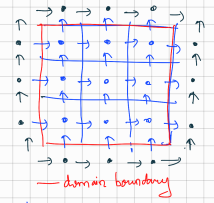
\includegraphics{bc.png}
    \caption{BC}
    \label{fig:BCs}
\end{figure}
Also, equate pressures outside and inside for a wall. Velocity perpendicular to the wall is 0. (no-slip).

With the concept of ghost cells Neumann boundary conditons can also be implemented as,
\begin{equation}
    \frac{\partial p}{\partial k} = b
\end{equation}
Choice of time step for the simulation is constrained by the Courant–Friedrichs–Lewy condition as explicit time discretization is used in the formulation. The Courant number is defined by 
\begin{equation}
Co = u * \delta{t}/\delta{x};
\end{equation}
Co should be less than 1 for stability. In the current simulation, the maximum non-dimensional velocity is 1 and non-dimensional dx is reciprocal of number of nodes. This gives us a bound for the dt.

\end{document}
